\documentclass[a4paper]{article}
\usepackage[spanish,es-tabla]{babel}	% trabajar en español
\spanishsignitems	
%\usepackage{simplemargins}

%\usepackage[square]{natbib}
\usepackage{amsmath}
\usepackage{amsfonts}
\usepackage{amssymb}
\usepackage{bbold}
\usepackage{graphicx}
\usepackage{blindtext}
\usepackage{hyperref}
\usepackage{amsthm}
\newtheorem{theorem}{Teorema}
\newtheorem{lemma}{Lema}



\begin{document}
\pagenumbering{arabic}

\Large
 \begin{center}
Tarea 3\\


\hspace{10pt}

% Author names and affiliations
\large
%Lic. Julio A. Medina$^1$ \\
Julio A. Medina$^1$ \\
\hspace{10pt}
\small  
$^1$ Universidad de San Carlos\\
Escuela de Ciencias Físicas y Matemáticas\\
Maestría en Física\\
\href{mailto:julioantonio.medina@gmail.com}{julioantonio.medina@gmail.com}\\

\end{center}

\hspace{10pt}

\normalsize
\section{Problema de valor inicial}
Resolver el siguiente problema de valor inicial
\begin{equation}
y''-2xy'-y=y^2 e^{-x^2}
\end{equation}
con condiciones de frontera
\begin{equation*}
y(0)=1,\,\,\,\,\,y'(0)=0
\end{equation*}
utilizando 2 pasos por el método de Runge Kutta, ver \cite{Burden}, con $h=0.5$ y $h=0.25$.\\
Para resolver este problema de valor inicial se ha implementado un script en c disponible en \url{https://github.com/Julio-Medina/Runge-Kutta/tree/main/code}\\
\begin{figure}[h]
\begin{center}
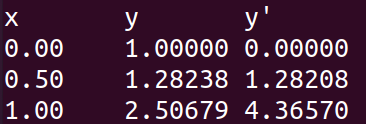
\includegraphics[scale=0.4]{./rkh05.png} 
\end{center} 
\caption{Resultado RK4 con $h=0.5$}
\label{plot}
\end{figure}
\begin{figure}[h]
\begin{center}
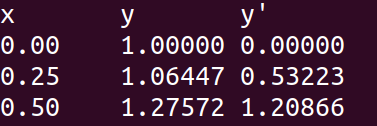
\includegraphics[scale=0.4]{./rkh025.png} 
\end{center} 
\caption{Resultado RK4 con $h=0.25$}
\label{plot}
\end{figure}



%En este trabajo de graduación consta de dos partes, en la primera parte se ha realizado una investigación sobre el enfoque de la mecánica estadística en la redes neuronales. En la segunda parte
\begin{thebibliography}{99}
%% La bibliografía se ordena en orden alfabético respecto al apellido del 
%% autor o autor principal
%% cada entrada tiene su formatado dependiendo si es libro, artículo,
%% tesis, contenido en la web, etc


\bibitem{Burden} Richard L. Burden, J. Douglas Faires \textit{Numerical Analysis}, (Ninth Edition). Brooks/Cole, Cengage Learning. 978-0-538-73351-9

%\bibitem{Feynman} 
%\bibitem{Hopfield} J.J. Hopfield. \textit{Neural Networks and physical systems with emergent collective computational abilities}. \url{https://doi.org/10.1073/pnas.79.8.2554}


%\bibitem{McCulloch} Warren S. McChulloch, Walter H. Pitts. \textit{A LOGICAL CALCULUS OF THE IDEAS IMMANENT IN NERVOUS ACTIVITY}. \url{http://www.cse.chalmers.se/~coquand/AUTOMATA/mcp.pdf}



\end{thebibliography}
\end{document}

